% !Mode\dots ``TeX:UTF-8''
% !TEX root = ../root.tex
\section{The online observability of \BCNs}
\label{sec:online}
In this section we propose the online observability, and introduced its related information in detail. We give the informal definition of it at first. 

%\begin{definition}
	A \BCN\ has online observability, iff its initial state $s_0$ can be determined in real time for every $s_0 \in \Delta_N$. In the online observability we determine the state of \BCN\ by dynamically observing its output sequence and then deriving and deciding the input sequence at every time step. And this process can be accomplished in finite time steps.
%\end{definition}  without presupposing the initial state of \BCN

The reason why we called this type of observability online observability is that:
\begin{itemize}
  \item First in this type of observability, we determine the initial state of \BCNs\ in real time. In other words, we can use one test case to determine the initial state of \BCNs. We call this property {\em real-time} property.%Such that we can determine the initial state of any test case of \BCNs.
  \item  Secondly in online observability, we use the outputs we observe to derive and decide the input sequence at every time step. By this way, we can make full use of the outputs to determine the initial state of \BCNs. We call this property {\em interactivity}.
\end{itemize} 

If we can determine the initial state of a biological system (depicted by \BCN) in real time, then we need only one test case to determine the initial state of it. Therefore we need the {\em real-time} property to help us avoid repeating biological experiments. And the {\em interactivity} would help us to find the necessary condition of determine the initial state of \BCNs\ in real time. With the  {\em real-time} and {\em interactivity}, we called this type of observability online observability.
%\tl{maybe I did not understand this, but I think you are confusing two things: the observability and the algorithm (approach) to determine the initial state. It seems to me that you are describing a new approach (the online approach), but does this change the observability? if yes, how? Is this a stronger notion or a weaker notion or incomparable?}

In order to make online observability satisfy real-time property and interactivity. In the left of this section, firstly we present the definition of derivation function. Secondly we present the definition of $k$-step determinability. We take them as the preparations for defining the online observability. Finally, we give the formal definition of the online observability of \BCNs. 
\subsection{Derivation function}
%Different from four existing observabilities, t
The observability we propose can determine the initial state online.
 %Because in the process of determining the initial state every input of the input sequence is decided by the output we observe at every time step. 
 In the time setp $k$, we observe the output of \BCNs\ at first. Through this we can infer the possible values of state-nodes and denote them by possible states set $S_k$. %Then as we can know the possible states set, 
 At the next step, we need to decide the input $i_k$ which satisfies that % will make sure any different possible states 
$s_i, s_j$ 
 will not turn into the same state after being affected by the input $i_k$ i.e., $Ls_i i_k\neq Ls_j i_k$ for any distinct $s_i, s_j\in S_k$. After deciding input, we can observe the new output, and then we can infer the new possible states set. The cardinal number of possible states set does not change or decrease in this process. We repeat the above process, if the cardinal number of possible states set turn into be $1$ then we can determine the state and the initial state of {\em BCN}. And the reason why the cardinal number of the possible states set would decrease will be shown in equation (\ref{equ:10}) and (\ref{equ:11}). 
 
To better describe the derivation process of a \BCN\'s initial state at every time step we mentioned above, we give a derivation function for it. The definition of this function is as follows.
\begin{definition}[Derivation Function] The derivation function can be defined as $\Ded\left(S, i, o\right)$. Using this function we can get a states set $\Ded\left(S, i, o\right)$ for $S$ after inputing $i$ and observing $o$. Therefore, based on derivation process mentioned before, we have that there exists the corresponding $s'\in S$ of $s$ such that 
%\[s=L\ltimes i\ltimes s'\ when\ i\neq \varepsilon, \] 

\[s=\left\{
\begin{array}{rcl}
L\ltimes i\ltimes s'      &      & {i\neq \varepsilon}\\
s'       &      & {i= \varepsilon}
\end{array} \right. \]

and 

\[H\ltimes s=o\ when\ o\neq \varepsilon, \]
for each element \[s\in \Ded\left(S, i, o\right)\]
\end{definition}
where   
\begin{itemize}
  \item $S\in 2^{\Delta_N}$ is the possible states set;
  \item $i\in (\Delta_M\cup\varepsilon)$ represents the input;
  \item $o\in(\Delta_Q\cup\varepsilon)$ represents the output; 
  \item $\Ded\left(S, i, o\right)\in 2^{\Delta_N}$ is the possible states set after derivation.
\end{itemize} 
 
 From the definition of derivation function, we have some equations for this function. For better illustration, we use the \BCN\ mentione earlier as an example. By researching these equations, we can know the details of this function better.
\begin{equation}
\begin{split}
\Ded\left(\emptyset,i,o\right)=\emptyset\\
%D\left(\varnothing,I_i,O_i\right)=D\left(\varnothing,\varepsilon,O_i\right)= &D\left(\varnothing,\varepsilon,\varepsilon\right)=\varnothing\\
\end{split}
\label{equ:7}
\end{equation}

Equation (\ref{equ:7}) represents that if the possible states set is an empty set $\emptyset$ then no matter what we input and observe, we can only deduce the possible set is $\emptyset$. It means that if we don't know anything about the state of a \BCN, then we can not deduce anything no matter what we do.
\begin{equation}
\begin{split}
\Ded\left(S,\varepsilon,\varepsilon\right)=&S\\
\end{split}
\label{equ:8}
\end{equation}

For any possible states set $S$ and we neither input anything and nor observe the output. In this case we can only deduce that the possible states set is $S$ shown in equation (\ref{equ:8}). It means that before inputing and observing the output of \BCN\ we can not know more information about this \BCN\ than we used to knew.
\begin{equation}
\begin{split}
\Ded\left(\Delta_N,\varepsilon,\delta_4^1\right)=&\{\delta_{16}^1,\delta_{16}^2,\delta_{16}^3\}\\
\end{split}
\label{equ:9}
\end{equation}
 
 Using the example mentioned before (\ref{equ:4}), when the possible states set $S=\Delta_N$, and  we observe that the outputs of \BCN\ is $\delta_4^1$ before we decide input. In this case we can deduce that the possible states would be $\delta_{16}^1$, $\delta_{16}^2$ or  $\delta_{16}^3$ shown in equation (\ref{equ:9}).
\begin{equation}
\begin{split}
\Ded\left(\{\delta_{16}^1,\delta_{16}^2,\delta_{16}^3\},\delta_4^1,\varepsilon\right)=&\{\delta_{16}^{10},\delta_{16}^4,\delta_{16}^{11}\}\\
\end{split}
\label{equ:10}
\end{equation}

And then, if the possible states set $S=\{\delta_{16}^1$, $\delta_{16}^2$, $\delta_{16}^3\}$ we input $\delta_4^1$. Before we observe the output of \BCN\ we can only deduce the possible states would be $\delta_{16}^{10}$, $\delta_{16}^4$ or  $\delta_{16}^{11}$ shown in equation (\ref{equ:10}). In other words, the cardinal number of the possible states set did not decrease before observing the output of this \BCN.
\begin{equation}
\begin{split}
\Ded\left(\{\delta_{16}^1,\delta_{16}^2,\delta_{16}^3\},\delta_4^1,\delta_4^3\right)=&\{\delta_{16}^{10},\delta_{16}^{11}\}\\
\end{split}
\label{equ:11}
\end{equation}

But if we observe that the output of \BCN\ is $\delta_4^3$, then we can deduce that the possible state can be $\delta_{16}^{10}$ or  $\delta_{16}^{11}$ shown in equation (\ref{equ:11}). Such that the cardinal number of the possible states set may decrease after observing the output of \BCN. Therefore, the derivation function helps the online obervability satisfy the {\em interactivity}.
\begin{equation}
\begin{split}
\Ded\left(\{\delta_{16}^4,\delta_{16}^5,\delta_{16}^6\},\delta_4^3,\varepsilon\right)=&\{\delta_{16}^9,\delta_{16}^{13}\}
\end{split}
\label{equ:12}
\end{equation}

 Finally if the set of possible states is $\{\delta_{16}^4,\delta_{16}^5,\delta_{16}^6\}$ and the inputs is $\delta_4^3$. Before we observe the output of \BCN\ we can deduce that the possible states should be $\delta_{16}^9$ or $\delta_{16}^{13}$ shown in equation (\ref{equ:12}). Because both $\delta_{16}^4$ and $\delta_{16}^5$ are turn into be the same state $\delta_{16}^9$ after affected by $\delta_4^3$. And if the current state of the \BCN\ is one of them then we can not determine the current state any more. We give a lemma to illustrate this rule.
\begin{lemma}
 In the time step $t$, $S$ is the set of current possible states we derived and $i(t)$ is the input we chose. If we can determine the current state $s(t)$ of this \BCN\ for every $s(t)\in S$, then we have 
 $|\Ded\left(S,i_p,\varepsilon\right)|=|S|$.
 \label{lemm:1}
\end{lemma}

\begin{proof}
In the time step $t$, $S$ is the set of current possible states we derived and $i(t)$ is the input we chose. And we can determine the current state $s(t)$ of this \BCN\ for every $s(t)\in S$. We assume that $|\Ded\left(S,i_p,\varepsilon\right)|<|S|$, then we have there exist $s_i(t), s_j(t)\in S$, $s_i(t)\neq s_j(t)$ that 
\[s_i(t+1)=L\ltimes i_p\ltimes s_i(t)=L\ltimes i_p\ltimes s_j(t)=s_j(t+1).\]
And then for any $p\in \mathbb{N}^*$ and fore any input sequence we chose, we have 
\[s_i(t+p)=s_j(t+p);\]
\[o_i(t+p)= H\ltimes{s_i(t+p)}= H\ltimes{s_j(t+p)}=o_j(t+p).\]
 Therefore we can not distinguish between $s_i(t)$ and $s_j(t)$ any more.
 If the current state is the $s_i(t)$ or $s_j(t)$, we can not determine it. But we can determine the current state $s(t)$ of this \BCN\ for every $s(t)\in S$, then the presumption $|\Ded\left(S,i_p,\varepsilon\right)|<|S|$ is wrong. So we have $|\Ded\left(S,i_p,\varepsilon\right)|=|S|$.
\end{proof}
 
% If the cardinality number of the possible states set of one \BCN\ decreased before observing its output the derivation process, then we can not deduce its initial state any more i.e., we can not determine the initial state of this \BCN\ any more. Therefore, the derivation function helps the online obervability satisfy the {\em real-time} property. 

As the derivation function can only describe the derivation process of a \BCN's initial state at every time step. But we need more than one time step to determine the initial state in general, thus we propose the $k$-step determinability to describe the whole process of determining a \BCN's initial state.
\subsection{$k$-step determinability}
After we difined the derivation function, we can present the definition of $k$-step determinability of the states set of \BCNs, where the $k\in \mathbb{N}$. It may easier to difine online observability by programming language. But we would like to define its mathematical form for preciseness of concepts. However, before defining the online observability of \BCNs, we need to difine the $k$-step determinability of the states set of \BCNs\ at first.
\begin{definition}[$k$-Step Determinability] 

When $k=0$, a set of states $S$ the $S$ is $0$-step deterministic if the cardinal number of this states set $|S|=1$. 

When $k>0$, a set of states $S$ is $k$-step deterministic
 if the cardinal number of this states set $|S|>1$, and for this set of states $S$ there exists $i_p \in \Delta_M$ such that
 \begin{itemize}
 \item  $|\Ded\left(S,i_p,\varepsilon\right)|=|S|$, and 
 \item  for each $o_j$ in $\Delta_Q$ such that $|\Ded\left(S,i_p,o_j\right)|\neq 0$ there exists a ${k'}<k$ that $\Ded\left(S,i_p,o_j\right)$ is $k'$-step deterministic.
 \end{itemize}
 %And we default $k\ge0$ when we talk about whether a states set of \BCNs\ $S$ is $k$-step deterministic or not.
\end{definition}

From the definition of {\em$k$}-step determinability we know that ``$k=0$'' means that we can determine the state without deciding any input and observing output. Because if we know the cardinality number of possible states set is $1$, then we can know the state of \BCNs. Therefore, we can only discuss the case of $k=0$ when $|S|=1$. If $k>0$, we have $|S|>1$. The formula $|\Ded\left(S,i_p,\varepsilon\right)|=|S|$ ensures that no different states will become the same state after being affected by the input $i_p$. Furthermore, the definition of $k$-step deterministic ( (k>0)) is defined recursively, and it need to use the definition of $k$-step deterministic ($k=0$) in the end. 
\begin{example}
In the previously mentioned \BCN. For the set of state $\{\delta_{16}^1,\delta_{16}^2,\delta_{16}^3\}$, the cardinality number of this set $|\{\delta_{16}^1,\delta_{16}^2,\delta_{16}^3\}|=3>1$, and for this set there exists $\delta_{4}^4$ such that 
 \begin{itemize}
 \item  $|\Ded\left(\{\delta_{16}^1,\delta_{16}^2,\delta_{16}^3\},\delta_{4}^4,\varepsilon\right)|=|\{\delta_{16}^1,\delta_{16}^2,\delta_{16}^3\}|$;
 \item  $|\Ded\left(\{\delta_{16}^1,\delta_{16}^2,\delta_{16}^3\},\delta_{4}^4,\delta_{4}^1\right)|=|\{\delta_{16}^1\}|=1$, and $\{\delta_{16}^1\}$ is $0$-step deterministic;
 \item  $|\Ded\left(\{\delta_{16}^1,\delta_{16}^2,\delta_{16}^3\},\delta_{4}^4,\delta_{4}^2\right)|=|\{\delta_{16}^7\}|=1$, and $\{\delta_{16}^7\}$ is $0$-step deterministic;
  \item  $|\Ded\left(\{\delta_{16}^1,\delta_{16}^2,\delta_{16}^3\},\delta_{4}^4,\delta_{4}^4\right)|=|\{\delta_{16}^14\}|=1$, and $\{\delta_{16}^14\}$ is $0$-step deterministic.
 \end{itemize}
 Therefore the set of states $\{\delta_{16}^1,\delta_{16}^2,\delta_{16}^3\}$ is $1$-step deterministic.
\end{example}  

What is more, we have some theorems for the $k$-step determinability.
\begin{lemma}
 In the time step $t$ and $S$ is the set of current possible states we derived. If $S$ is $k$-step deterministic, then we can determine the current state $s(t)$ of this \BCN\ for every $s(t)\in S$ in time step $t+k$.
  \label{lemm:6}
\end{lemma}
\begin{proof} If $k=0$, then we have $|S|=1$ that we can determine the current state $s(t)$ of this \BCN\ in time step $t$. Therefore the {\em Lemma \ref{lemm:6}} is right. If for $k=0,\ldots k=p$ the {\em Lemma \ref{lemm:6}} is right. When $k=p+1$ we have for this set of states $S$ there exists $i_p \in \Delta_M$ such that
 \begin{itemize}
 \item  $|\Ded\left(S,i_p,\varepsilon\right)|=|S|$, and 
 \item  for each $o_j$ in $\Delta_Q$ such that $|\Ded\left(S,i_p,o_j\right)|\neq 0$ there exists a ${k'}<k$ that $\Ded\left(S,i_p,o_j\right)$ is $k'$-step deterministic.
 \end{itemize}
 Therefore we can determine the state $s(t+1)$ of this \BCN\ for every $s(t+1)\in \Ded\left(S,i_p,\varepsilon\right)$ in time step $t+k$. What is more, $|\Ded\left(S,i_p,\varepsilon\right)|=|S|$ then for every $s(t+1)\in \Ded\left(S,i_p,\varepsilon\right)$ we can find the corresponding one $s(t)$ for it. So we can determine the state $s(t)$ of this \BCN\ for every $s(t)\in S$ in time step $t+k$. And then we have if for $k=0,\ldots k=p$ the {\em Lemma \ref{lemm:6}} is right then the {\em Lemma \ref{lemm:6}} is right too when $k=p+1$. Moreover, the lemma is right when $k=0$, so we have for any $k\in \mathbb{N}$ the {\em Lemma \ref{lemm:6}} is right.
\end{proof}
\begin{lemma}
 In the time step $t$ and $S$ is the set of current possible states we derived. If we can determine the current state $s(t)$ of this \BCN\ for every $s(t)\in S$ in time step $t+k$, then $S$ is $k$-step deterministic.
  \label{lemm:7}
\end{lemma}

\begin{proof}
In the time step $t$ and $S$ is the set of current possible states we derived. 
When $k=0$ and we can determine the current state $s(t)$ of this \BCN\ for every $s(t)\in S$ in time step $t$, then we have $|S|=1$, $S$ is $0$-step deterministic. Therefore, we have the {\em Lemma \ref{lemm:7}} is right when $k=0$. If for $k=0,\ldots k=p$ the {\em Lemma \ref{lemm:7}} is right. When $k=p+1$, from the {\em Lemma \ref{lemm:1}} we have for this set of states $S$ there exists $i_p \in \Delta_M$ such that
 \begin{itemize}
 \item  $|\Ded\left(S,i_p,\varepsilon\right)|=|S|$, and 
 \item  for each $o_j$ in $\Delta_Q$ such that $|\Ded\left(S,i_p,o_j\right)|\neq 0$ there exists a ${k'}<(p+1)$ that $\Ded\left(S,i_p,o_j\right)$ is $k'$-step deterministic.
 \end{itemize} Therefore, we have $S$ is $p+1$-step deterministic. And then have if for $k=0,\ldots k=p$ the {\em Lemma \ref{lemm:7}} is right then the {\em Lemma \ref{lemm:7}} is right too when $k=p+1$. Moreover, the lemma is right when $k=0$, so we have for any $k\in \mathbb{N}$ the {\em Lemma \ref{lemm:7}} is right.
\end{proof}

We can consider the ``A $S$ is $k$-step deterministic'' as ``We can determine the state of a \BCN\ by this possible states set $S$ in $k$ steps, and we finish this determination process by deciding input sequence and observing out sequence at each time step.'' Therefore if we can determine the infimum of $k$ for a set of states $S$, we would find the length of the shortest path to determine the state of a \BCN\ by this possible states set $S$.
\begin{lemma}
 If a set of states $S$ is $k_1$-step deterministic and $k_1< k_2$, then $S$ is $k_2$-step deterministic. But if the states set $S$ is $k_1$-step deterministic and $k_1> k_2$, we can not deduce that $S$ is $k_2$-step deterministic. 
  \label{lemm:2}
\end{lemma}

\begin{proof}
 A set of states $S$ is $k_1$-step deterministic and the $k_1< k_2$. 
 
 If $k_1=0$ then $|S|=1$. Therefore for this set of states $S$ there exists $i_p$ in $\Delta_M$ such that
 \begin{itemize}
 \item  $|\Ded\left(S,i_p,\varepsilon\right)|=|S|=1$, and 
 \item  for each $o_j$ in $\Delta_Q$ such that $|\Ded\left(S,i_p,o_j\right)|\neq 0$ and $\Ded\left(S,i_p,o_j\right)$ is $k'$-step deterministic with  ${k'}=0=k_1< k_2$.
 \end{itemize}
 Therefore the set of states $S$ is $k_2$-step deterministic.
 
 If $k_1>0$, then $|S|>1$. Therefore for this set of states $S$ there exists $i_p$ in $\Delta_M$ such that
 \begin{itemize}
 \item  $|\Ded\left(S,i_p,\varepsilon\right)|=|S|$, and 
 \item  for each $o_j$ in $\Delta_Q$ such that $|\Ded\left(S,i_p,o_j\right)|\neq 0$ and $\Ded\left(S,i_p,o_j\right)$ is $k'$-step deterministic with  ${k'}<k_1< k_2$.
 \end{itemize}
 Therefore the set of states $S$ is $k_2$-step deterministic.

 But if the states set $S$ is $k_1$-step deterministic and $k_1> k_2$. What is more, for this set of states $S$ there is no such $i_p$ in $\Delta_M$ such that
 \begin{itemize}
 \item  $|\Ded\left(S,i_p,\varepsilon\right)|=|S|$, and 
 \item  for each $o_j$ in $\Delta_Q$ such that $|\Ded\left(S,i_p,o_j\right)|\neq 0$ and $\Ded\left(S,i_p,o_j\right)$ is $k'$-step deterministic with  ${k'}<k_2<k_1$.
 \end{itemize}
 Therefore the set of states $S$ is not $k_2$-step deterministic.
 
 So we have the {\em Lemma \ref{lemm:2}} is right.
\end{proof}

\begin{definition}[$k_{inf}(S)$] 
If for a set of states $S$, there exists a $k_i\in \mathbb{N}$ such that $S$ is $k_i$-step deterministic but $S$ is not $(k_{i}-1)$-step deterministic, then $k_{i}$ is the $k_{inf}(S)$.
\end{definition}

In {\em Section \ref{sec:app}}, we will present the details on selecting the shortest path when we use the online observability to determine the initial state of a \BCN. 


%{\em Theorem \ref{theo:4}}

We can consider ``A set of possible states $S$ is $K$-step deterministic'' as ``We can determine the state of a \BCN\ by this possible states set $S$ in finite steps''. Therefore we have some other theorems for the $K$-step determinability.



We prove the {\em Lemma \ref{lemm:4}} at first.
\begin{lemma}
 If a set of states $S_j$ is $k$-step deterministic and $S_i\subset S_j$, then $S_i$ is $k$-step deterministic, where $|S_j|>1$.
  \label{lemm:4}
\end{lemma}
\begin{proof}
A set of states $S_j$ is $k$-step deterministic and $S_i\subset S_j$, where $|S_j|>1$. Therefore we have $k>0$ in this precondition.

If $k=1$, we have for this set of states $S_j$ there exists $i_p$ in $\Delta_M$ such that
 \begin{itemize}
 \item  $|\Ded\left(S_j,i_p,\varepsilon\right)|=|S_j|$, and 
 \item  for each $o_j$ in $\Delta_Q$ such that $|\Ded\left(S_j,i_p,o_j\right)|=1\neq 0$ and $\Ded\left(S_j,i_p,o_j\right)$ is $0$-step deterministic.
 \end{itemize}
 Then we have for the set of states $S_i$ there exists $i_p$ in $\Delta_M$ such that
 \begin{itemize}
 \item  $|\Ded\left(S_i,i_p,\varepsilon\right)|=|S_i|$, and 
 \item  for each $o_j$ in $\Delta_Q$ such that $|\Ded\left(S_i,i_p,o_j\right)|=1\neq 0$ and $\Ded\left(S_i,i_p,o_j\right)$ is $0$-step deterministic.
 \end{itemize} And then $S_i$ is $k$-step deterministic, we have the {\em Lemma \ref{lemm:4}} is right when $k=1$.
 
 If for $k=1,\ldots k=p$ the {\em Lemma \ref{lemm:4}} is right. When $k=p+1$, we have  for this set of states $S_j$ there exists $i_p$ in $\Delta_M$ such that
 \begin{itemize}
 \item  $|\Ded\left(S_j,i_p,\varepsilon\right)|=|S_j|$, and 
 \item  for each $o_j$ in $\Delta_Q$ such that $|\Ded\left(S_j,i_p,o_j\right)|\neq 0$ and $\Ded\left(S_j,i_p,o_j\right)$ is $k'$-step deterministic with  ${k'}<(p+1)$.
 \end{itemize}
 Then we have for the set of states $S_i$ there exists $i_p$ in $\Delta_M$ such that
 \begin{itemize}
 \item  $|\Ded\left(S_i,i_p,\varepsilon\right)|=|S_i|$, and 
 \item  for each $o_j$ in $\Delta_Q$ such that $|\Ded\left(S_i,i_p,o_j\right)| \le |\Ded\left(S_j,i_p,o_j\right)|\neq 0$ and $\Ded\left(S_i,i_p,o_j\right)\subset \Ded\left(S_j,i_p,o_j\right)$ is  $k'$-step deterministic with  ${k'}<(p+1)$.
 \end{itemize}  And then $S_i$ is $k$-step deterministic. Therefore we have if for $k=1,\ldots k=p$ the {\em Lemma \ref{lemm:4}} is right, then the {\em Lemma \ref{lemm:4}} is right when $k=p+1$. What is more, we have the {\em Lemma \ref{lemm:4}} is right when $k=1$, thus the {\em Lemma \ref{lemm:4}} is right for any $k\in\mathbb{N}$
\end{proof}

\subsection{Online observability}
After the previous preparation, we present the formal definition of the online observability. The formal definition of the online observability of {\em BCNs} is as follows.
Since we don't need to find the the specific value of $k$ when we define the online observability by $k$-step determinability, we defined the concept of $K$-Step Determinability for convenience.
\begin{definition}[$K$-Step Determinability] 
If for a set of states $S$, there exists a $k_i\in \mathbb{N}$ such that $S$ is $k_i$-step deterministic, then it is $K$-step deterministic.
\end{definition}

\begin{definition}[Online Observability of  BCNs]
 A \BCN\ is online observable,
if for every  $o_j$ in $\Delta_Q$ such that $|\Ded\left(\Delta_N,\varepsilon, o_j\right)|\neq 0$, the $\Ded\left(\Delta_N,\varepsilon,o_j\right)$ is $K$-step deterministic.
% We even can define the online observability simpler, if there exists $k \ge 0$ implies $\Delta_N$ is $k$ stepes deterministic, then this \BCN\ is online observable. 
\end{definition}

%The difference between the second definition and the first definition is that whether we observe the corresponding output of the initial state of \BCN\ at first. For better performance, we use the first definition of online observability.

\begin{example}
In the previously mentioned \BCN. We have:
 \begin{itemize}
 \item $|\Ded\left(\Delta_N,\varepsilon, \delta_{4}^1\right)|=\{\delta_{16}^1,\delta_{16}^2,\delta_{16}^3\}\neq 0$, and it is $1$-step deterministic;
 \item $|\Ded\left(\Delta_N,\varepsilon, \delta_{4}^2\right)|=\{\delta_{16}^4,\delta_{16}^5,\delta_{16}^6,\delta_{16}^7\}\neq 0$, and it is $1$-step deterministic;
 \item $|\Ded\left(\Delta_N,\varepsilon, \delta_{4}^3\right)|=\{\delta_{16}^8,\delta_{16}^9,\delta_{16}^{10},\delta_{16}^{11}\}\neq 0$, and it is $2$-step deterministic;
 \item $|\Ded\left(\Delta_N,\varepsilon, \delta_{4}^4\right)|=\{\delta_{16}^{12},\delta_{16}^{13},\delta_{16}^{14},\delta_{16}^{15},\delta_{16}^{16}\}\neq 0$, and it is $2$-step deterministic.
 \end{itemize}
 
Therefore we have this \BCN\ satisfies the online observability.
\end{example}  

From the informal definition and formal definition of online observability, we have a theorem for it. 
\begin{theorem}
The necessary and sufficient condition of determine the initial state $s_0$ of \BCNs\ for every $s_0\in \Delta_N$ in real time is the online observability of \BCNs. 
\label{theo:1}
\end{theorem}
\begin{proof}
 A \BCN\ is online observable,
then for every  $o_j$ in $\Delta_Q$ such that $|\Ded\left(\Delta_N,\varepsilon, o_j\right)|\neq 0$, the $\Ded\left(\Delta_N,\varepsilon,o_j\right)$ is $K$-step deterministic. From the {\em Lemma \ref{lemm:6}} and the $\Ded\left(\Delta_N,\varepsilon,o_j\right)$ is $K$-step deterministic, then we have there exists a $k_i$ such that we can determine the $s_o$ in time step $k_i$ for every $s_0\in \Ded\left(\Delta_N,\varepsilon,o_j\right)$.  What is more for every  $o_j$ in $\Delta_Q$ such that $|\Ded\left(\Delta_N,\varepsilon, o_j\right)|\neq 0$, the $\Ded\left(\Delta_N,\varepsilon,o_j\right)$ is $K$-step deterministic, then we have there exists a $k_i$ such that we can determine the $s_o$ in time step $k_i$ for every $s_0\in \Delta_N$. Therefore we can determine the initial state $s_0$ of \BCNs\ for every $s_0\in \Delta_N$ in real time.

If we can determine the initial state $s_0$ of \BCNs\ for every $s_0\in \Delta_N$ in real time. From the {\em Lemma \ref{lemm:7}}, and for any set of initial possible states $\Ded\left(\Delta_N,\varepsilon,o_j\right)$ we derived, there exists a $k_i$ such that we can determine the $s_o$ in time step $k_i$ for every $s_0\in \Ded\left(\Delta_N,\varepsilon,o_j\right)$, we have  $\Ded\left(\Delta_N,\varepsilon,o_j\right)$ is $k_i$-step deterministic and then $K$-step deterministic, therefore this \BCN\ is online observable.

So we have the {\em Theorem \ref{theo:1}} is right.
\end{proof}
%With the online observability we can find the best way we like to determine the initial state of \BCNs.
\begin{lemma}
 If a set of states $S_j$ is $K$-step deterministic and $S_i\subset S_j$, then $S_i$ is $K$-step deterministic, where $|S_j|>1$.
\label{lemm:3}
\end{lemma}
\begin{proof}A set of states $S_j$ is $K$-step deterministic and $S_i\subset S_j$. Then there exists a $k_i\in \mathbb{N}$ such that $S_j$ is $k_i$-step deterministic. By the {\em Lemma \ref{lemm:4}}, we have $S_i$ is $k_i$-step deterministic too. And then we have the $S_i$ is $K$-step deterministic as well.
\end{proof}

With the {\em Lemma \ref{lemm:3}}, we would have its equivalent proposition is right as well.
\begin{lemma}
 If a set of states $S_i$ is not $K$-step deterministic and $S_i\subset S_j$, then $S_j$ is not $K$-step deterministic. 
  \label{lemm:5}
\end{lemma}
\begin{proof}
A set of states $S_i$ is not $K$-step deterministic and $S_i\subset S_j$. If the set of states $S_j$ is $K$-step deterministic we have $S_i$ is $K$-step deterministic too. But $S_i$ is not $K$-step deterministic, therefore we have $S_j$ is not $K$-step deterministic.
\end{proof}
\subsection{Online observability and existing observability}
After defining online observability of \BCNs, we discuss the comparison of online observability with the four existing observability. In the existing second type of observability, we presuppose the initial state of a \BCN, and then try to find the input sequence to distinguish it from other types of initial state. But the input sequence determined by the presupposed initial state may make some other types of initial state turn into be the same state (equation \ref{equ:12}). Such that some of other types of initial states can not be distinguished anymore, and if the initial state of this \BCN\ is one of them then the initial state can not be determined anymore. This problem has to be considered in the online obervability of \BCNs. Hence we have a theorem for online observability and the existing first and second observability.
\begin{theorem}
If a \BCN\ satisfies the online obervability then it satisfies the existing first and second observability. If a \BCN\ satisfies the existing first or second observability we can not deduce that it satisfies the online obervability.
\end{theorem}
\begin{proof}
 If a set of states $S$ is $k_1$-step deterministic and $k_1\leq k_2$, then $S$ is $k_2$-step deterministic. But if the states set $S$ is $k_1$-step deterministic and $k_1\geq k_2$, we can not deduce that $S$ is $k_2$-step deterministic. 
\end{proof}

In the existing third type of observability, there has to exist an input sequence that can distinguish any distinct states. However in online observability we can use different input sequences to distinguish any distinct states in different sets of state. 
%Where these different sets of state are classified by their corresponding outputs. Therefore, we have the existing third type of observability implies the online observability of \BCNs, then the existing fourth type of observability implies the online observability too. 
\begin{theorem}
If a \BCN\ satisfies the existing third or fourth obervability then it satisfies the online observability. But if a \BCN\ satisfies the online obervability, we can neither deduce that it satisfies the third observability nor deduce that it satisfies the fourth observability.
\end{theorem}
\begin{proof}
 If a set of states $S$ is $k_1$-step deterministic and $k_1\leq k_2$, then $S$ is $k_2$-step deterministic. But if the states set $S$ is $k_1$-step deterministic and $k_1\geq k_2$, we can not deduce that $S$ is $k_2$-step deterministic. 
\end{proof}

The implication relationships graph between four existing observability and online observability is shown in Fig.\ref{fig:7}.
%\begin{example}
%For instance, the \BCN\ whose structure is depicted in Fig.\ref{fig:1}, and the updating rules of this \BCN\ is described as truth table in Fig.\ref{fig:2}. This \BCN\ satisfies the existing first, second, third observability, but it is not satisfy the existing fourth observability. Therefore, we have this \BCN\ satisfies the online observability from the implication relationship between the existing third observability and online observability.
%\end{example}   

\begin{figure}[thpb]
      \centering
      \framebox{\parbox{3in}{
		\centerline{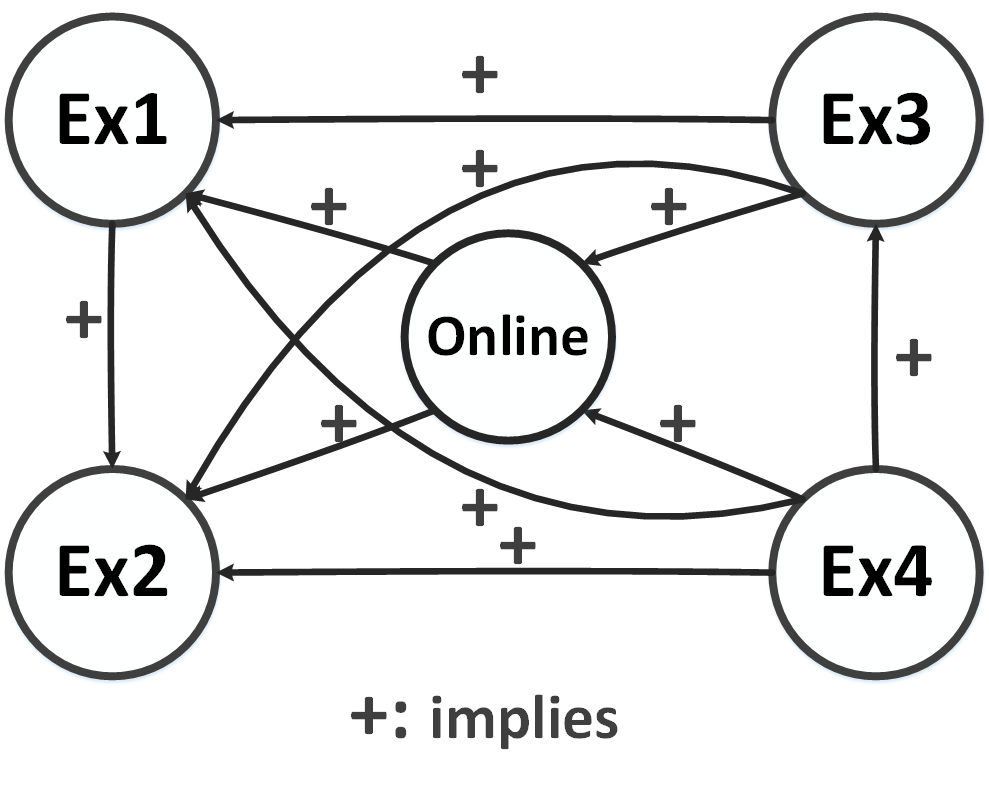
\includegraphics[scale=0.28]{figures/Fig8.png}}
	}}
      
      \caption{The implication relationships graph between existing observability 1, 2, 3, 4, and online observability where ``+" means ``implies".}
      \label{fig:7}
   \end{figure}
   
%When I learned the four existing kinds of observability of \BCNs, I found that if we want to determine the initial state of a \BCN\ by first kind of observability, we need to guess the initial state of the \BCN\ and then check it by its corresponding input sequence. If the initial state we guess is right then we can determine the initial state of this \BCN. But if what we guess is incorrect, we need to guess the initial state again and use its corresponding input sequence to determine the initial state of this \BCN. We repeat this process untll we determine the initial state of this \BCN. But if we can not repeat this process, we can not determine the initial state of the \BCN\ too. Then I turned my gaze to the third observability, this kind of observability makes we can determine the initial state without presupposing the initial state. But I thought if we can determine the possible states set of the \BCN\ by observing the output at first, why do not we find corresponding input sequences for these possible states sets when we determine the initial state of \BCN? Compared with the existing third observability this method needs weaker preconditions of \BCNs\ for us to determine their initial state. Then I talked about this thinkness with my teacher, and we expand it into the original idea of the online observability of \BCNs. 
%==============================================================================================================